\begin{appendices}
\addtocontents{toc}{\protect\setcounter{tocdepth}{2}}\makeatletter
\addtocontents{toc}{%
  \begingroup
  \let\protect\l@chapter\protect\l@section
  \let\protect\l@section\protect\l@subsection
}
\makeatother


\section{General deployment diagram}\label{app:deployment-diagram}
\begin{landscape}
   \begin{figure}
    \centering
    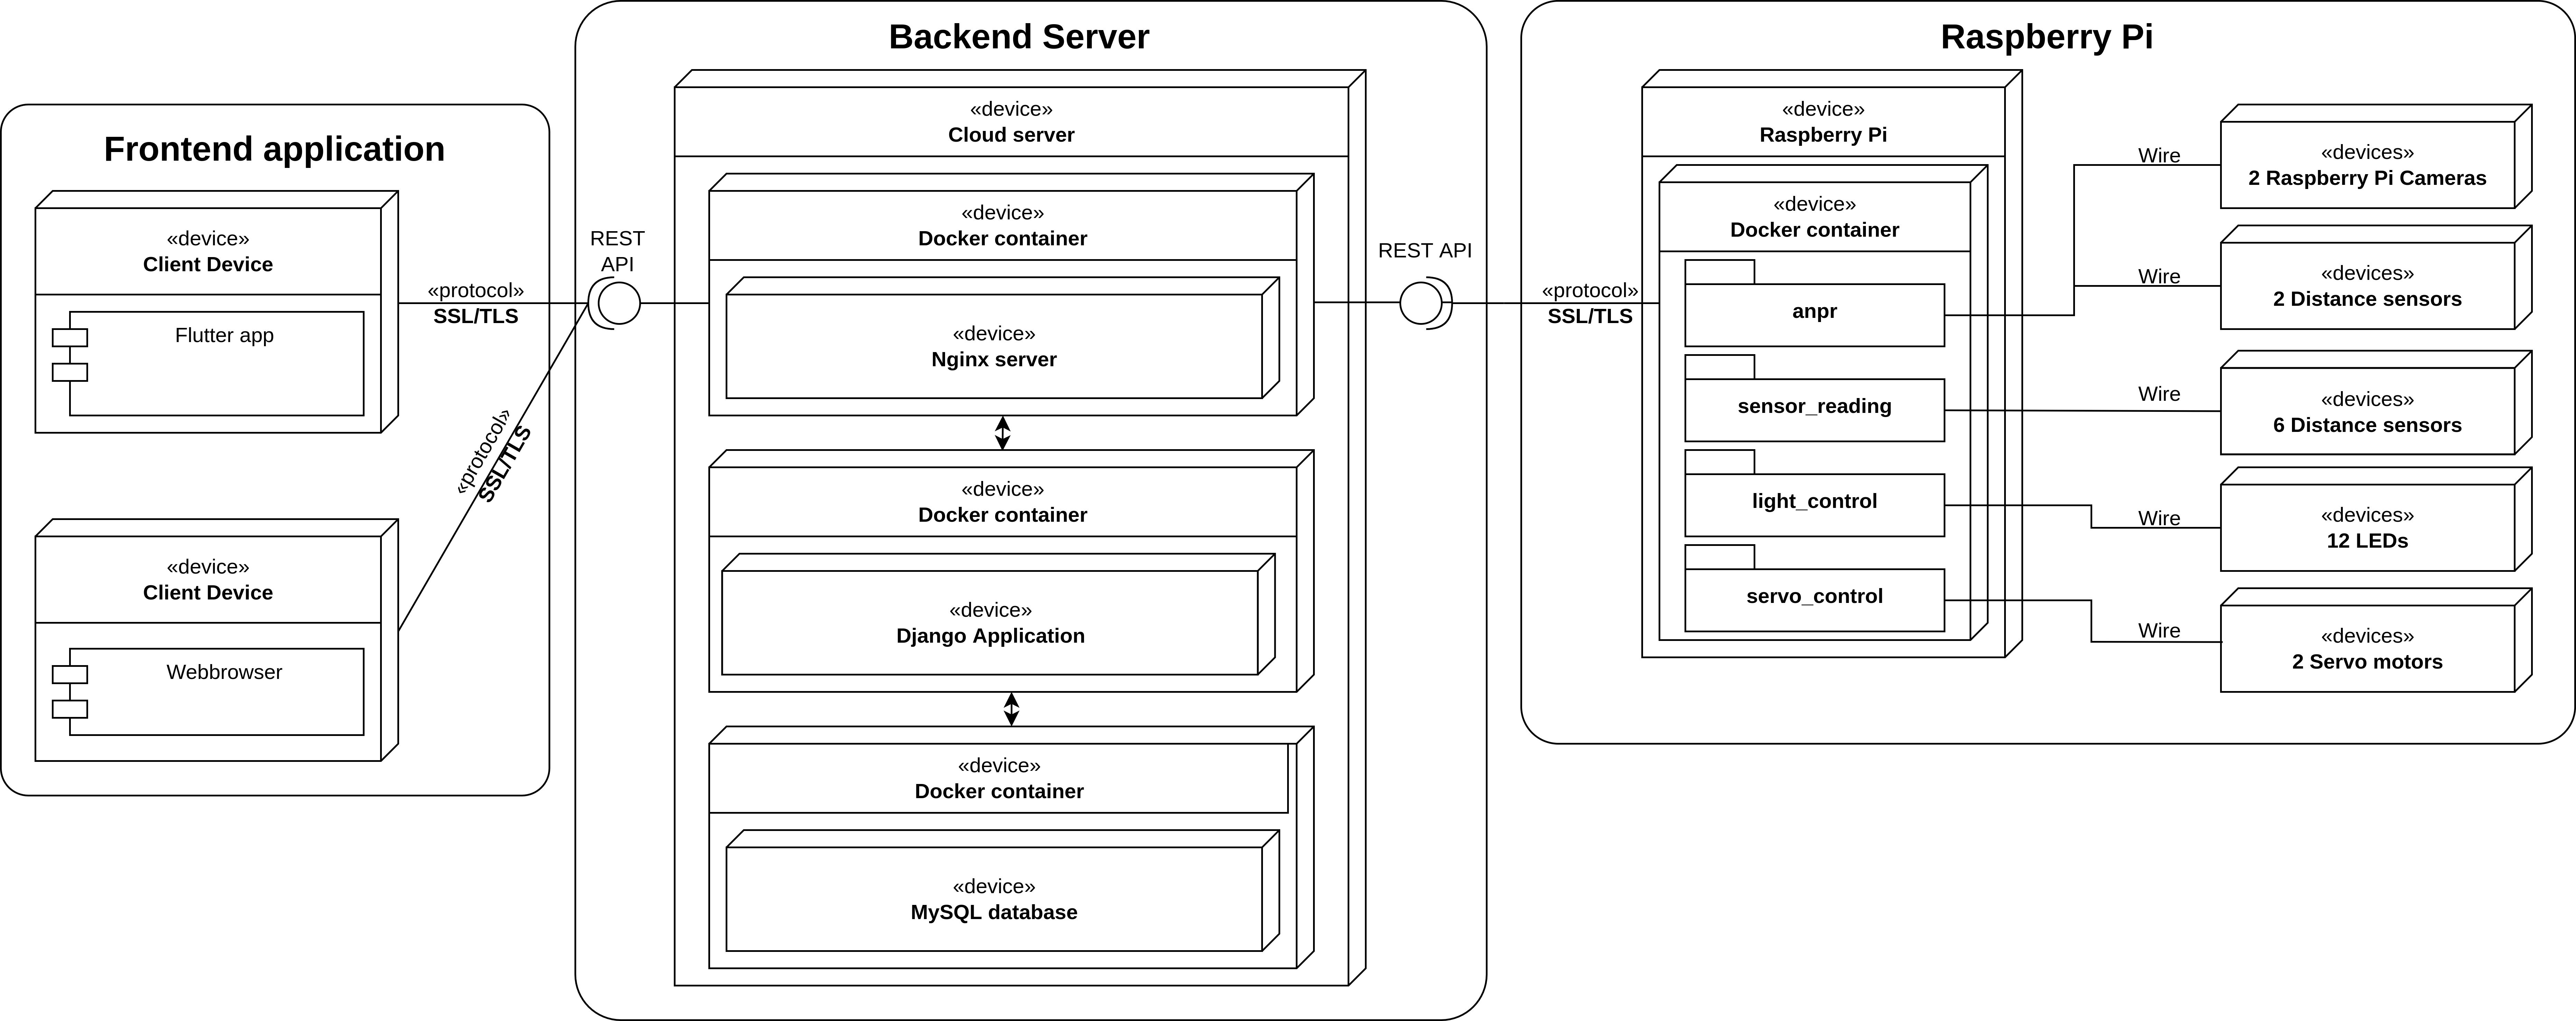
\includegraphics[width=25cm]{images/deployment_diagram.drawio.png}
    \caption{General deployment diagram.}
    \label{fig:general-deployment-diagram}
\end{figure}
\end{landscape}

\clearpage


\section{Application design}\label{app:app-design}
\begin{figure}[htp]
    \centering
    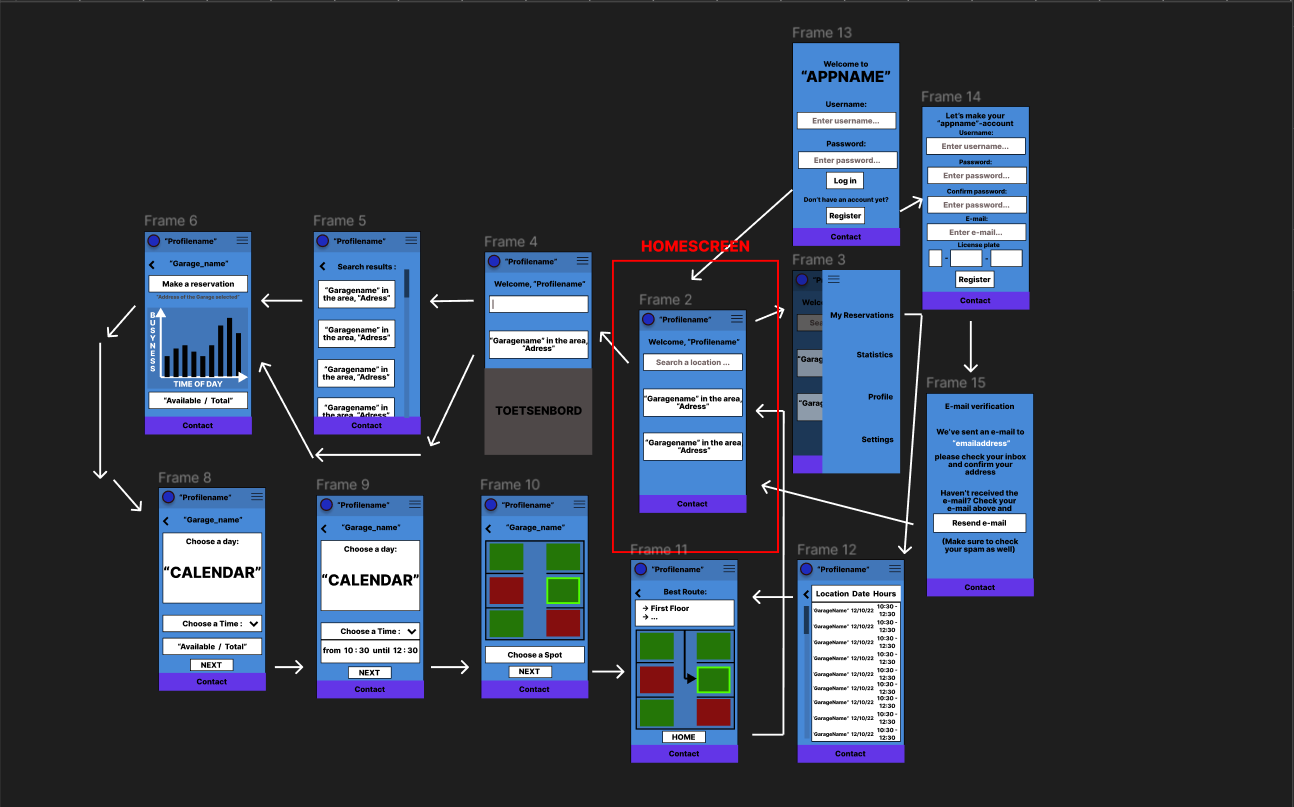
\includegraphics[width=16cm]{images/AppDesign.png}
    \caption{Current app design.}
    \label{fig:AppDesign}
\end{figure}

\section{Mechanical part list}\label{app:part-list}

\begin{table}[htp]
    \centering
    \caption{Overview of all used mechanical components and their model number.}
    \begin{tabular}{|c|c|c|}
        \hline
         \textbf{Component name} & \textbf{Model number} & \textbf{Amount}  \\
         \hline
         Raspberry Pi & Model 3B & 1 \\
         \hline
         \textsc{dorhea} Raspberry Pi Mini Kamera & \textsc{he0304-002} & 2 \\
         \hline
         Ultrasonic distance measuring sensor & \textsc{hc-sr04} & 8 \\
         \hline
         \textsc{Micro servo motor} & \textsc{oky8003} & 2 \\
         \hline
         Red \textsc{led} ($3 \ \text{mm}$) & \textsc{com-00533} & 6 \\
         \hline
         Green \textsc{led} ($3 \ \text{mm}$) & \textsc{com-09560} & 6 \\
         \hline
         Resistors ($20 \ \text{k}\Omega$) & \textsc{sfr2500002002fr500} & 12 \\
         \hline
         Jumper cables & / & $\approx 60$ \\
         \hline
         Raspberry Pi camera extension cable & \textsc{b087dfJ2rp} & 2 \\
         \hline
         \end{tabular}
    \label{tab:part_list}
\end{table}
\clearpage

\section{Flowcharts}\label{app:flowcharts}

\begin{figure}[htp]
    \centering
    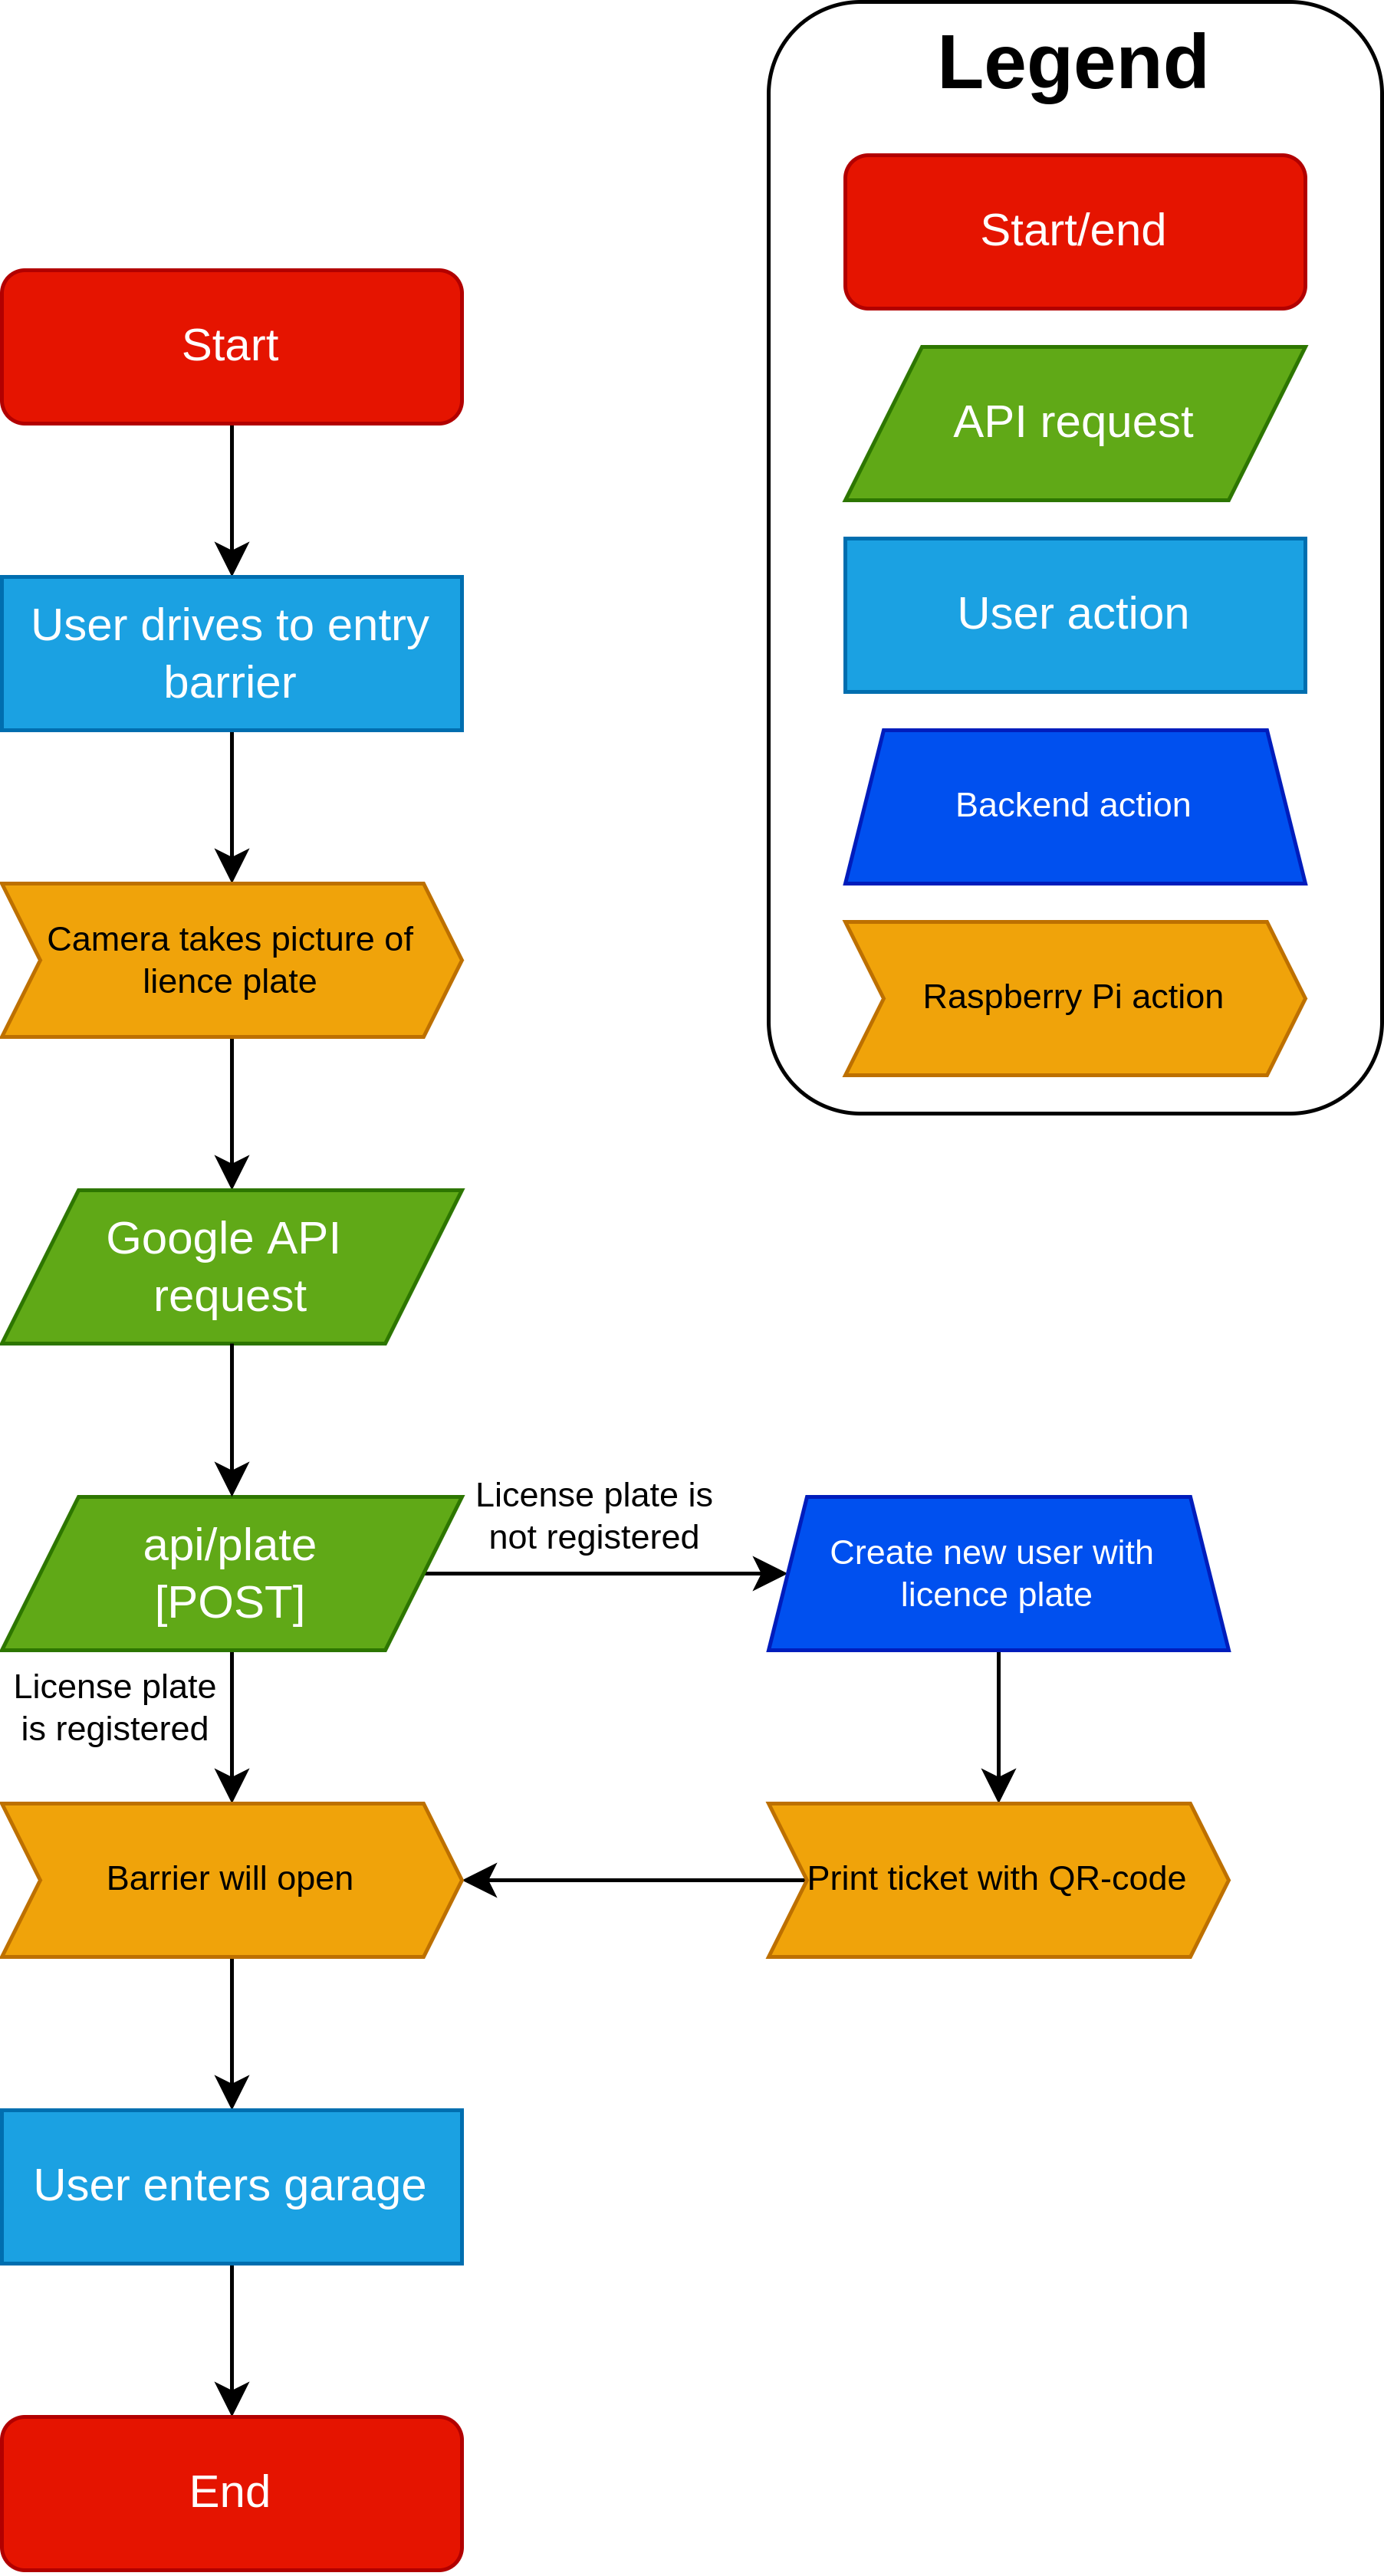
\includegraphics[width=7cm]{images/garage_enter.drawio.png}
    \caption{Flowchart of the entering process of the garage in both hardware, software and user terms.}
    \label{fig:garage-enter}
\end{figure}

\begin{figure}[htp]
    \centering
    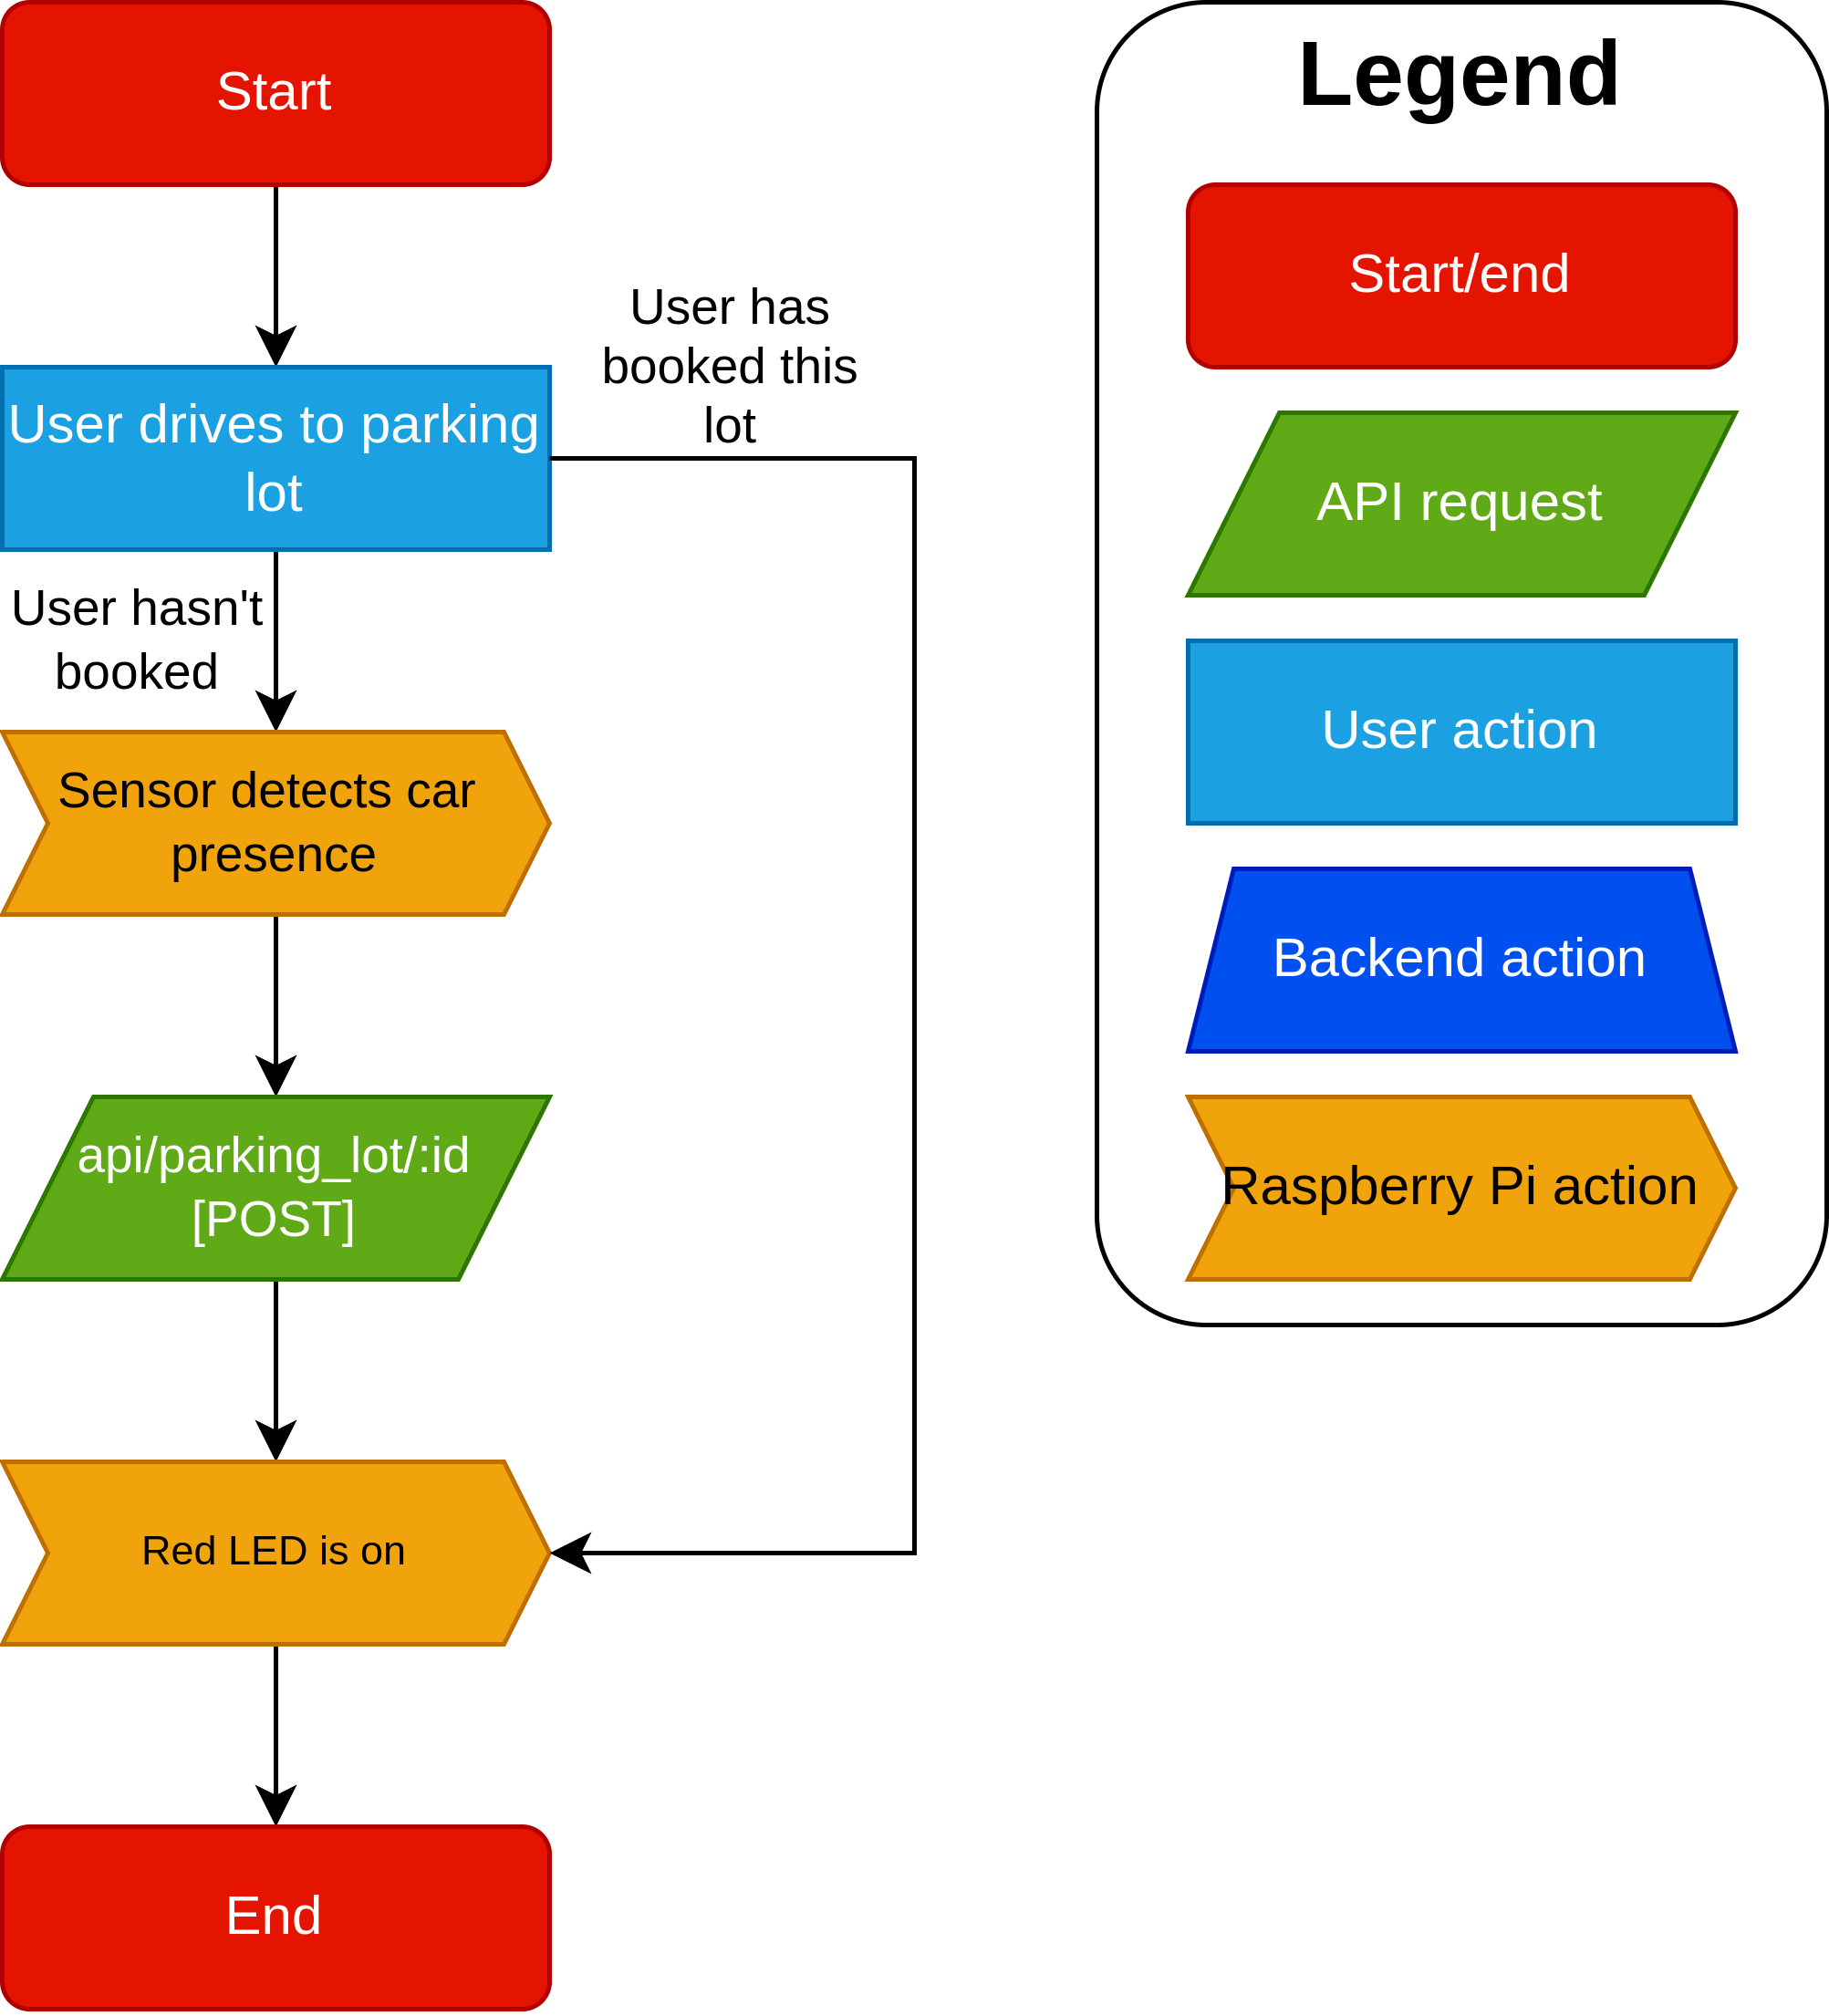
\includegraphics[width=7cm]{images/car_detection.drawio.png}
    \caption{Flowchart of the car detection process of the garage in both hardware, software and user terms.}
    \label{fig:car-detection}
\end{figure}

\begin{figure}[htp]
    \centering
    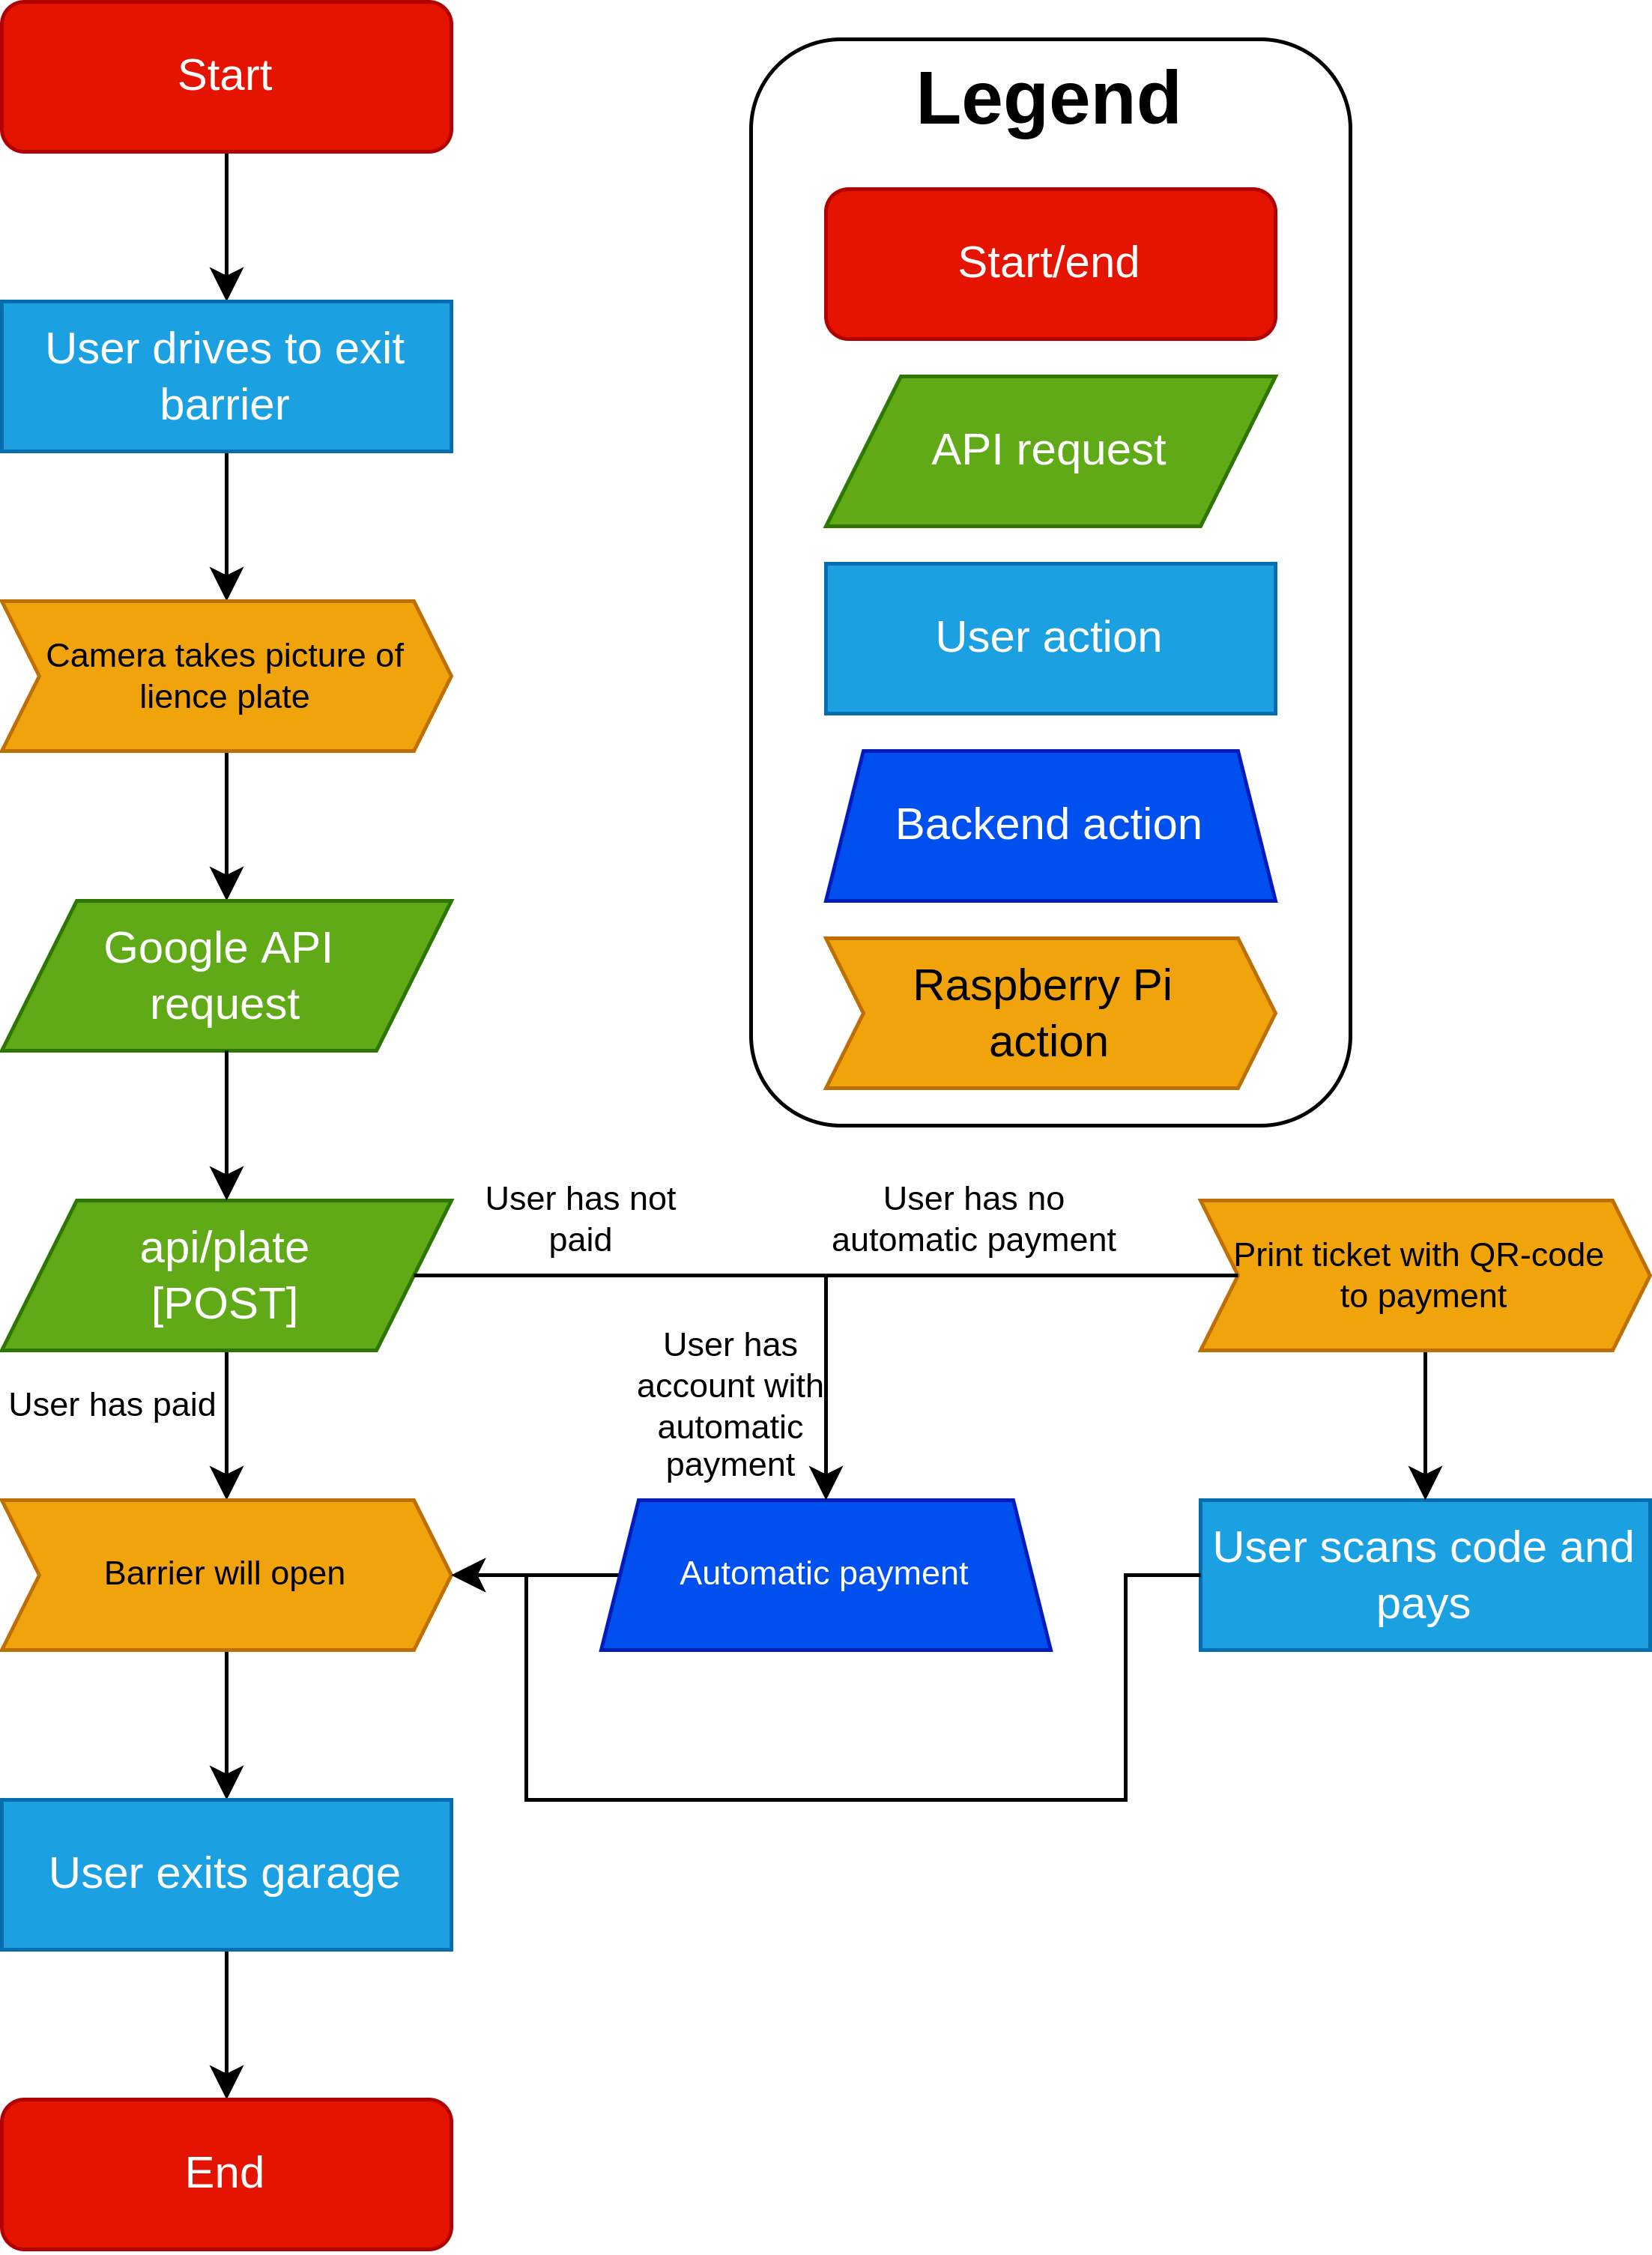
\includegraphics[width=8cm]{images/garage_exit.drawio.png}
    \caption{Flowchart of the exiting process of the garage in both hardware, software and user terms.}
    \label{fig:garage-exit}
\end{figure}


\end{appendices}
